\section{Almindelige trigonometriske identiteter}

\subsection{Omregning mellem grader og radianer}

\subsubsection{Grader til radianer}
For at gå fra en vinkel i grader $\theta_{\text{grad}}$ til en vinkel i radianer $\theta_{\text{rad}}$ kan følgende formel benyttes
\[ 
\theta_{\text{rad}} = \theta_{\text{grad}} \cdot \frac{\pi}{180}
.\]

\subsubsection{Radianer til grader}
For at gå fra en vinkel i radianer $\theta_{\text{rad}}$ til en vinkel i grader $\theta_{\text{grad}}$ kan følgende formel benyttes
\[ 
\theta_{\text{grad}} = \theta_{\text{rad}} \cdot \frac{180}{\pi}
.\]


\subsection{Omregning mellem trigonometriske funktioner}
\begin{figure} [ht]
  \centering
  \caption{Hver af de trigonometriske funktioner skrevet afhængigt af hver af de 5 andre}
  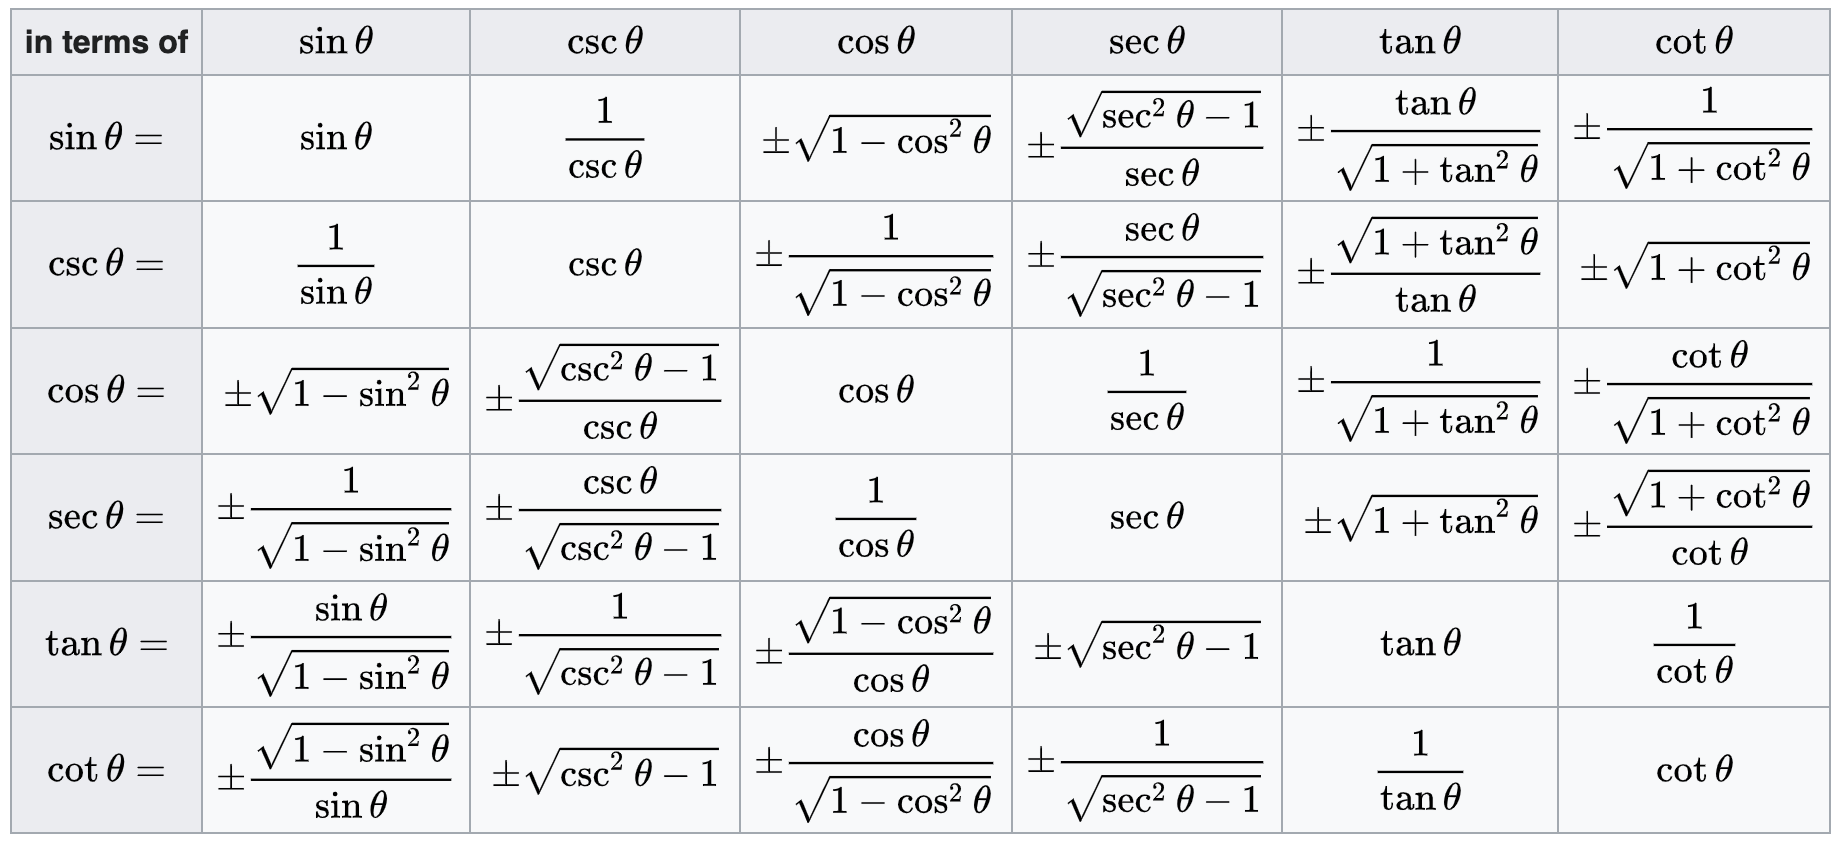
\includegraphics[width=0.8\linewidth]{../figures/trig_id.png}
  \label{fig:trig_id}
\end{figure}

På \textbf{\autoref{fig:trig_id}} ses en omregningstabel, hvor hver af de trigonometriske funktioner er givet afhængigt af hver af de 5 andre.

\subsection{Den pythagoræiske identitet (idiotformlen)}
Den pythagoræiske identitet foreskriver at
\[ 
\sin^2 \theta + \cos^2 \theta = 1
.\]

\subsection{Eksakte værdier af de trigonometriske funktioner}
\begin{figure} [ht]
  \centering
  \caption{Eksakte værdier af de trigonometriske funktioner for almindelige vinkler}
  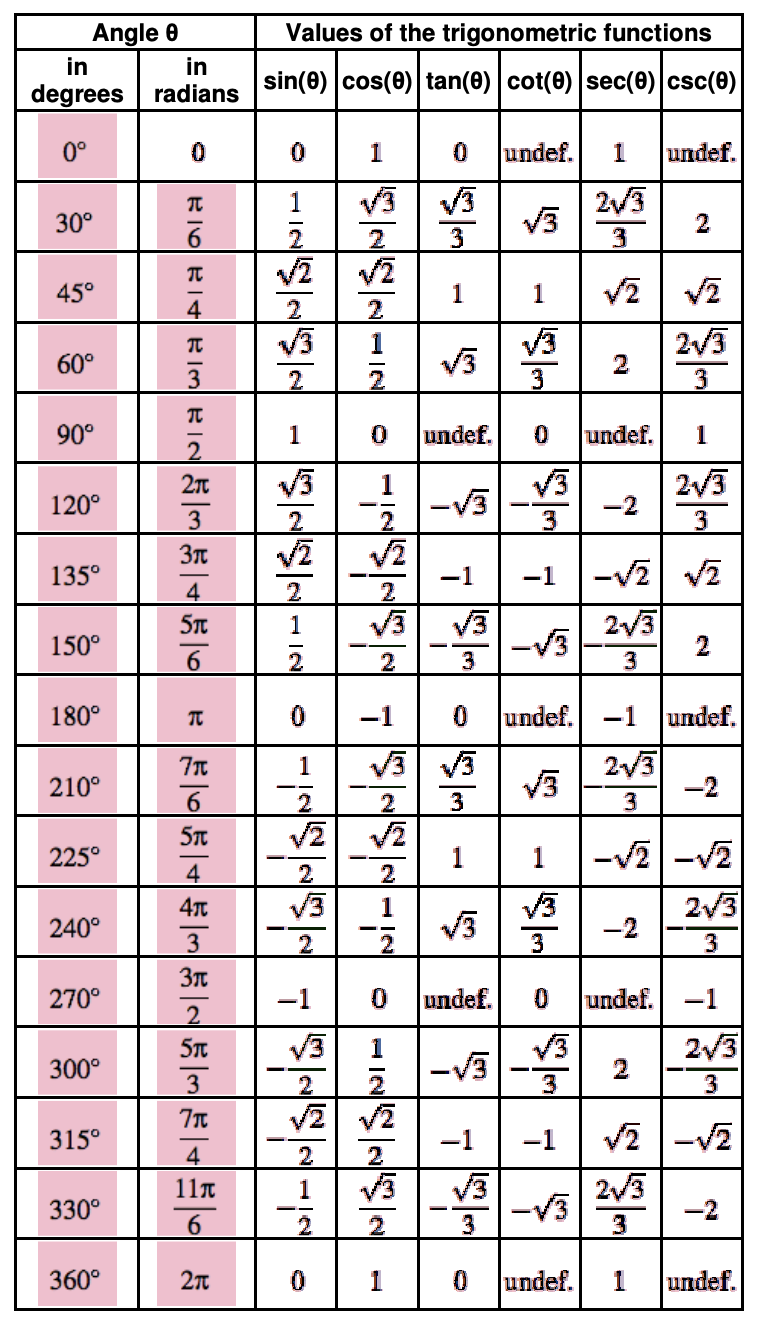
\includegraphics[width=0.75\linewidth]{../figures/trig_fun.png}
  \label{fig:trig_fun}
\end{figure}

På \textbf{\autoref{fig:trig_fun}} ses en oversigt over de eksakte værdier af de trigonometriske funktioner for de mest almindelige vinkler.

\clearpage

\subsection{Sammenligning af vinkler}
\begin{figure} [ht]
  \centering
  \caption{\textit{Cheat Sheet} til sammenligning af vinkler}
  \includegraphics[width=0.5\linewidth]{../figures/vinkelsammenligninger.png}
  \label{fig:vinkelsammenligninger}
\end{figure}

På \textbf{\autoref{fig:vinkelsammenligninger}} ses en oversigt hvilke vinkler der er ens.


\newpage

